\documentclass[tikz,border=10pt]{standalone}

\usepackage{amsmath,amssymb}
\usepackage{tikz}
\usetikzlibrary{arrows.meta,positioning,calc,fit}

\newcommand{\F}{\mathbb{F}}
\newcommand{\ol}[1]{\overline{#1}}

\begin{document}
	
	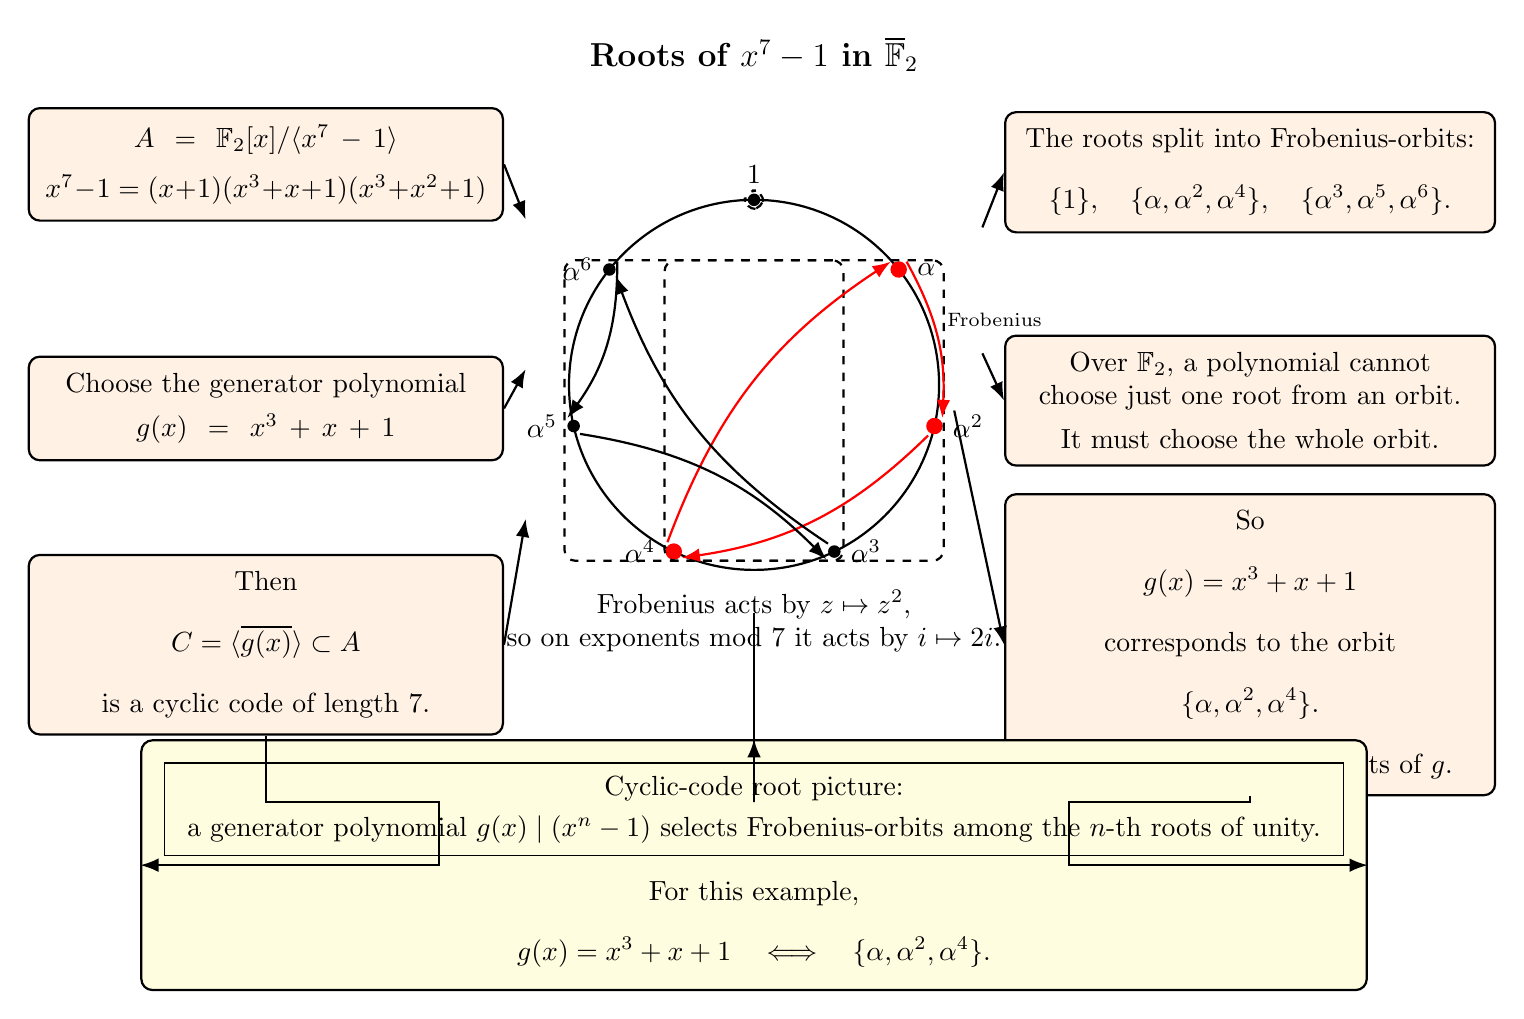
\begin{tikzpicture}[
		>=Latex,
		panel/.style={draw, rounded corners, thick, inner sep=8pt},
		box/.style={draw, rounded corners, thick, fill=orange!10, align=center, inner sep=6pt},
		note/.style={align=center},
		orbitbox/.style={draw, dashed, thick, rounded corners},
		root/.style={circle, fill=black, inner sep=1.6pt},
		selectedroot/.style={circle, fill=red, inner sep=2.1pt}
		]
		
		% --------------------------------------------------
		% Left algebra box
		% --------------------------------------------------
		\node[box, text width=5.6cm] (A) at (-6.2,3.6) {%
			$A=\F_2[x]/\langle x^7-1\rangle$\\[6pt]
			$x^7-1=(x+1)(x^3+x+1)(x^3+x^2+1)$
		};
		
		\node[box, text width=5.6cm] (G) at (-6.2,0.5) {%
			Choose the generator polynomial\\[4pt]
			$g(x)=x^3+x+1$
		};
		
		\node[box, text width=5.6cm] (C) at (-6.2,-2.5) {%
			Then
			\[
			C=\langle \ol{g(x)}\rangle \subset A
			\]
			is a cyclic code of length $7$.
		};
		
		% --------------------------------------------------
		% Middle geometric circle
		% --------------------------------------------------
		\node[font=\bfseries\large] at (0,5.0) {Roots of $x^7-1$ in $\overline{\F}_2$};
		
		\coordinate (O) at (0,0.8);
		\def\r{2.35}
		
		\draw[thick] (O) circle (\r);
		
		% 7th roots positions
		\coordinate (P0) at ($(O)+(90:\r)$);
		\coordinate (P1) at ($(O)+(38.571:\r)$);
		\coordinate (P2) at ($(O)+(-12.857:\r)$);
		\coordinate (P3) at ($(O)+(-64.286:\r)$);
		\coordinate (P4) at ($(O)+(-115.714:\r)$);
		\coordinate (P5) at ($(O)+(-167.143:\r)$);
		\coordinate (P6) at ($(O)+(141.429:\r)$);
		
		% Draw all roots
		\node[root,label=above:$1$] at (P0) {};
		\node[selectedroot,label=right:$\alpha$] at (P1) {};
		\node[selectedroot,label=right:$\alpha^2$] at (P2) {};
		\node[root,label=right:$\alpha^3$] at (P3) {};
		\node[selectedroot,label=left:$\alpha^4$] at (P4) {};
		\node[root,label=left:$\alpha^5$] at (P5) {};
		\node[root,label=left:$\alpha^6$] at (P6) {};
		
		% Orbit boxes
		\node[orbitbox, fit=(P0)] (Orb0) {};
		\node[orbitbox, fit=(P1)(P2)(P4)] (Orb1) {};
		\node[orbitbox, fit=(P3)(P5)(P6)] (Orb2) {};
		
		\node[note] at ($(O)+(0,-3.0)$) {%
			Frobenius acts by $z\mapsto z^2$,\\
			so on exponents mod $7$ it acts by $i\mapsto 2i$.
		};
		
		% Frobenius arrows on selected orbit
		\draw[->, thick, red] ($(P1)+(0.10,0.10)$) to[bend left=16] node[above right, black] {\scriptsize Frobenius} ($(P2)+(0.10,0.10)$);
		\draw[->, thick, red] ($(P2)+(-0.08,-0.12)$) to[bend left=18] ($(P4)+(0.10,-0.08)$);
		\draw[->, thick, red] ($(P4)+(-0.08,0.12)$) to[bend left=18] ($(P1)+(-0.10,0.10)$);
		
		% Frobenius arrows on other orbit
		\draw[->, thick] ($(P3)+(-0.08,0.10)$) to[bend left=18] ($(P6)+(0.08,-0.08)$);
		\draw[->, thick] ($(P6)+(0.10,0.10)$) to[bend left=18] ($(P5)+(-0.08,0.10)$);
		\draw[->, thick] ($(P5)+(0.08,-0.10)$) to[bend left=18] ($(P3)+(-0.10,-0.10)$);
		
		% --------------------------------------------------
		% Right explanation boxes
		% --------------------------------------------------
		\node[box, text width=5.8cm] (R1) at (6.3,3.5) {%
			The roots split into Frobenius-orbits:
			\[
			\{1\},\quad
			\{\alpha,\alpha^2,\alpha^4\},\quad
			\{\alpha^3,\alpha^5,\alpha^6\}.
			\]
		};
		
		\node[box, text width=5.8cm] (R2) at (6.3,0.6) {%
			Over $\F_2$, a polynomial cannot choose just one root from an orbit.\\[4pt]
			It must choose the whole orbit.
		};
		
		\node[box, text width=5.8cm] (R3) at (6.3,-2.5) {%
			So
			\[
			g(x)=x^3+x+1
			\]
			corresponds to the orbit
			\[
			\{\alpha,\alpha^2,\alpha^4\}.
			\]
			The red points are the roots of $g$.
		};
		
		% --------------------------------------------------
		% Bottom summary
		% --------------------------------------------------
		\node[
		draw,
		rounded corners,
		thick,
		fill=yellow!12,
		text width=15.0cm,
		align=center,
		inner sep=8pt
		] (S) at (0,-5.3) {%
			$\boxed{
				\begin{array}{c}
					\text{Cyclic-code root picture:}\\[3pt]
					\text{a generator polynomial } g(x)\mid (x^n-1)
					\text{ selects Frobenius-orbits among the }n\text{-th roots of unity.}
				\end{array}
			}$\\[8pt]
			For this example,
			\[
			g(x)=x^3+x+1
			\quad\Longleftrightarrow\quad
			\{\alpha,\alpha^2,\alpha^4\}.
			\]
		};
		
		% --------------------------------------------------
		% Connecting arrows
		% --------------------------------------------------
		\draw[->, thick] (A.east) -- ($(O)+(-2.9,2.1)$);
		\draw[->, thick] (G.east) -- ($(O)+(-2.9,0.2)$);
		\draw[->, thick] (C.east) -- ($(O)+(-2.9,-1.7)$);
		
		\draw[->, thick] ($(O)+(2.9,2.0)$) -- (R1.west);
		\draw[->, thick] ($(O)+(2.9,0.4)$) -- (R2.west);
		\draw[->, thick] ($(Orb1.east)+(0.12,0)$) -- (R3.west);
		
		\draw[->, thick] (C.south) |- (-4.0,-4.5) |- (S.west);
		\draw[->, thick] ($(O)+(0,-2.9)$) -- (0,-4.5) -- (S.north);
		\draw[->, thick] (R3.south) |- (4.0,-4.5) |- (S.east);
		
	\end{tikzpicture}
	
\end{document}